\documentclass[a4paper,12pt]{article}
\usepackage{xspace}
\usepackage{tikz}
\newcommand\mT{\mathcal{T}}
\newcommand\T{$\mT$\xspace}
\newcommand\Tp{$\mT'$\xspace}
\newcommand\mtp{\models_{\mT'}}
\newcommand\syms{\mathop{\mathit{syms}}}
\title{Interpolation in SMTInterpol 2.0}
\author{J{\"u}rgen Christ \and Jochen Hoenicke}
\date{2012/06/30}
\begin{document}
\maketitle
\section{General Remarks}
SMTInterpol interpolates against some background theories and their extensions.
If \T is a theory and $\Gamma$ are assumptions not part of the interpolation
problem, then SMTInterpol computes interpolants against $\mT\wedge\Gamma$.

SMTInterpol computes a series of interpolants:
Given a theory extension \Tp and an interpolation problem
$A_0,\ldots,A_n,B$ such that $A_0\wedge\ldots\wedge A_n\wedge B$ is
unsatisfiable modulo \Tp, we produce $n+1$ interpolants $I_0,\ldots,I_n$ such
that
\begin{itemize}
\item $\bigwedge_{i=0}^mA_i\mtp I_m$, for all $0\le m\le n$
\item $\bigwedge_{i=m+1}^nA_i\wedge B\wedge I_m\mtp\bot$, for all $0\le m\le n$
\item $\syms(I_m)\subseteq(\bigcup_{i=0}^m\syms(A_i))\cap
  (\bigcup_{i=m+1}^n\syms(A_i)\cup\syms(B))$, for all $0\le m\le n$
\end{itemize}
\section{Interpolation in SMTLIB 1.2}
SMTInterpol accepts input in SMTLIB version 1.2 format benchmark files.
The special marker
\begin{verbatim}
:notes "Interpolation Problem starts here"
\end{verbatim}
is used to separate the theory extension from the interpolation problem.
If this marker is not present, no interpolants are computed.

Every assumption or formula after the marker is considered one part of the
interpolation problem.
The parts are added in the same order they appear in the input file.

The example below shows an interpolation problem against the theory of
uninterpreted functions extended with a sort consisting of exactly two element.

\begin{verbatim}
(benchmark twopointuniverse.smt
:logic AUFLIA
:extrasorts ((U))
:extrafuns ((a U)(b U)(s1 U)(s2 U)(c1 U)(c2 U))
:assumption (forall (?x U) (or (= ?x c1) (= ?x c2)))
:assumption (distinct c1 c2)
:notes "Interpolation problem starts here"
:assumption (= a s1)
:assumption (distinct s1 s2)
:formula (and (distinct b s1) (distinct b s2)))
\end{verbatim}

The example above produces two interpolants modulo the theory of uninterpreted
functions and linear integer arithmetic extended with the two-elementary sort
$U$:
\begin{enumerate}
\item $\top$ for $A\equiv a = s1$ and $B\equiv s1\ne s2\wedge(b\ne s1\wedge
  b\ne s2)$ and
\item $s1 \ne s2$ for $A\equiv a = s1\wedge s1\ne s2$ and $B\equiv(b\ne
  s1\wedge b\ne s2)$.
\end{enumerate}

\section {Interpolation in SMTLIB 2.0}

We propose one new option \texttt{:produce-interpolants} and one new
command \texttt{get-interpolants} for SMTLIB version 2 script format.
The option should be set before the \texttt{set-logic} command to tell
the solver that the user is interested in interpolants.  The
\texttt{get-interpolants} command is only supported if the option is
set to \textbf{true}. 

\emph{Rationale.} For performance reasons a solver can omit the proof
tracking necessary to compute interpolants unless this option was set.
To ease solver implementation we do not allow this option to be
changed after the \texttt{set-logic} command.

To compute Craig interpolants the interpolation problem must first be
given via \texttt{assert} commands and checked for unsatisfiability
using \texttt{check-sat}.  The asserted formulas should have a
\texttt{:named} annotation that provides a name to the formula, i.e., 
the formulas are asserted in the form
\begin{verbatim}
  (assert (! formula :named some_name))
\end{verbatim}
The name is referenced in the \texttt{get-interpolants} call.  
%
The simplest form of this call is
\begin{verbatim}
  (get-interpolants A B)
\end{verbatim}
where \texttt{A} and \texttt{B} are the names of the formulas for which
the interpolant should be computed.  The solver should reply with a
parenthesised \emph{term} that represents an interpolant for $A$ and
$B$, i.\,e., a formula with
\begin{itemize}
\item $A \land \lnot I$ is unsatisfiable.
\item $I \land B$ is unsatisfiable.
\item $I$ contains only the symbols shared between $A$ and $B$ or
  theory defined symbols.
\end{itemize}

\emph{Rationale.} This syntax is similar to the way the command
\texttt{get-unsat-core} works.  In both cases, the formulas are given
\texttt{:named} annotations and asserted and the unsatisfiability is
checked before-hand using \texttt{check-sat}.  The difference is that
for unsat cores the names are used in the result, while for
interpolation they are used as input to the command.

Separating \texttt{check-sat} and \texttt{get-interpolants} also
allows to compute several interpolants (with different partitions) for
the same formula.

The parenthesis around the answer become clear when considering the
extension for computing a sequence of interpolants.

\subsection{Theory extensions}
All unnamed formulas and all named formulas that are not mentioned in
the \texttt{get-interpolation} command are considered to be theory
extensions.  Thus the unsatisfiability of the formulas $A\land \lnot
I$ and $I\land B$ need only to hold in the context of the other
formulas.  Also $I$ may contain any symbol occuring in an unnamed
formula.

\subsection{Inductive Sequences of Interpolants}
As a simple extension \texttt{get-interpolants} can also be called
with more than two named formulas.  The reply to the command
\begin{verbatim}
  (get-interpolant F1 F2 ... Fn)
\end{verbatim}
should be a parenthesised sequence of $n-1$ interpolants 
\verb+(I1 I2 ... In-1)+, where
\begin{itemize}
\item $F_1\land \lnot I_1$ is unsat,
\item $I_i\land F_i \land \lnot I_{i+1}$ is unsat for $1\leq i \leq n-2$, and
\item $I_n\land F_n$ is unsat.
\item $I_i$ contains only the symbols that occur in one of the
  formulas $F_1,\dots,F_{i-1}$ and in one of the formulas
  $F_i,\dots,F_n$.  Again, symbols that occur in any unmentioned
  formula (theory extension) are also allowed.
\end{itemize}

\subsection{Tree Interpolants}

Let $T=(V,E)$ be a tree with a labelling $F : V \to \mathit{term}$
that assigns to each vertex a formula.  McMillan defines the tree
interpolants~\cite{z3 homepage} as a second labelling $I: V\to
\mathit{term}$ that assigns to each vertex an interpolant.  The
condition for the interpolants are:
\begin{itemize}
\item
  If the children of $v_i$ are $v_{j_1},\dots,v_{j_n}$, then
  \[I(v_{j_1})\land \dots \land I(v_{j_n}) \land F(v_i) \land \lnot I(v_i) \mbox{ is unsat},\]
  i.\,e., the formula of a vertex and the interpolants of its children imply the
  interpolant of the vertex.
\item The root vertex $r$ is labelled with the interpolant
  $I(r)=\mathtt{false}$.
\item The interpolant of a vertex $v$ may only contain symbols that occur
  in some input formula in the subtree starting with node $v$ and in
  some input formula that is not in the subtree starting with node $v$.
\end{itemize}

Tree interpolants are a generalization of nested
interpolants~\cite{TODO} and are useful for programs with procedures.
They can also be useful for more general class of programs where
verification conditions are expressible by Horn clauses.  This
includes parallel programs, object oriented programs and many more.

A sequence of interpolants can be seen as as special case of a tree
interpolant for the tree
\[ F_1 \longleftarrow F_2 \longleftarrow \cdots \longleftarrow F_n,\]
where $F_n$ is the root of the tree and $I_i$ is the interpolants of
the vertex labelled with $F_i$.  This suggests that the encoding of
the trees should be such that the above tree is encoded by the
sequence \verb+F1 F2 ... Fn+.  We propose the following EBNF
to encode a tree:

\def\nt#1{\mathop{\mathit{#1}}} % <\mbox{#1}>

\begin{eqnarray*}
  \nt{tree}&::=&\nt{symbol}\mathrel{|}\nt{subtrees} \nt{symbol}\\
  \nt{subtrees}&::=&\nt{tree} \mathrel{|} \nt{tree} ( \nt{subtrees} ) \\
\end{eqnarray*}

The non-terminal $\nt{symbol}$ matches a name of a named
formula.  The first rule encodes a tree as either a single symbol (for
a single-node tree) or as the encoding of the subtrees of the root
vertex followed by the symbol labelling the root vertex.  The encoding
of the first child requires no parenthesis (thus yielding in the
simple encoding for a sequence), but its siblings need to be
parenthesised to encode the tree structure.  Note that the grammar
above is LALR(1) and should be easy to parse.  The formulas appear in
the same order as in a post-order traversal of the tree.
%
\begin{figure}
  \begin{center}
  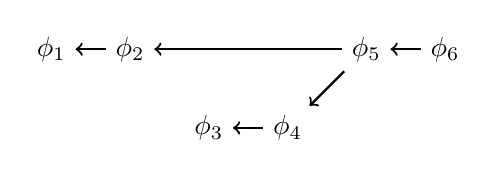
\begin{tikzpicture}[rotate=90]
    \node (xz) at (0,0) {$\phi_1$};
    \node (call) at (0,-1) {$\phi_2$};
    \node (s)  at(-1,-2) {$\phi_3$};
    \node (rx)  at(-1,-3) {$\phi_4$};
    \node (ret)  at(0,-4) {$\phi_5$};
    \node (assert)  at(0,-5) {$\phi_6$};
    \draw[thick, <-] (xz) -- (call);
    \draw[thick, <-] (s) -- (rx);
    \draw[thick, <-] (rx) -- (ret);
    \draw[thick, <-] (ret) -- (assert);
    \draw[thick, <-] (call) -- (ret);
  \end{tikzpicture}
  \end{center}
  \caption{\label{fig:treeipex}Example Formula Tree}
\end{figure}
%
E.\,g., to compute the interpolants for the tree depicted in
Figure~\ref{fig:treeipex}, the command is
\begin{verbatim}
(get-interpolants phi1 phi2 (phi3 phi4) phi5 phi6)
\end{verbatim}

The solver replies to this command with a parenthesised sequence of
interpolants \texttt{(I1 I2 \dots In-1)} that correspond to the
post-order traversal of the tree.  The last interpolant, which is the
interpolant \texttt{false} annotated to the root vertex, is omitted
from the returned sequence.  The tree structure is also omitted from
the output.

\subsection{Combining Partitions}

Sometimes it may be useful to combine two named formulas into a single
partition without computing an intermediate interpolant between these
formulas.  Instead of a single name of a formula, SMTInterpol also allows to combine several formulas with \texttt{and}.  E.g. to compute the interpolant for $A=\phi_1$ and $B=\phi_2 \land \phi_3$, the following command can be used:
\begin{verbatim}
(get-interpolants phi1 (and phi2 phi3))
\end{verbatim}

\emph{Caveat.}  This may lead to confusion with the parenthesis used
in tree interpolants.  Since \texttt{and} cannot be used as name of a
formula, the grammar is still unambiguous, but it is a bit more tricky
to build an LALR grammar.  Also note that this requires \texttt{and} to
be a keyword, which it is not in the current SMTLIB 2 standard.  

For this reason I will not strongly vote for including the
\texttt{and}-extension in the standard.  The use-cases for which we
needed them are superseeded by the tree interpolants.

\subsection{Example}
Next example shows the SMTLIB 2.0 counterpart of the previous example.
Again, we compute two interpolants modulo the theory of integer linear
arithmetic and uninterpreted functions extended with a two element sort $U$.
The example also shows the intermixing of theory extension and interpolation
problem.
Answers from the solver are given below the command and are preceded by a
semicolon.

{\footnotesize\begin{verbatim}
(set-option :print-success false)
(set-option :produce-interpolants true)
(set-logic QF_UFLIA)
(declare-fun x_1 () Int)
(declare-fun xm1 () Int)
(declare-fun x2 () Int)
(declare-fun res4 () Int)
(declare-fun resm5 () Int)
(declare-fun xm6 () Int)
(declare-fun x7 () Int)
(declare-fun res9 () Int)
(declare-fun resm10 () Int)
(declare-fun res11 () Int)
(assert (! (<= x_1 100) :named M1))
(assert (! (= xm1 (+ x_1 11)) :named M2))
(assert (! (> x2 100) :named S11))
(assert (! (= res4 (- x2 10)) :named S12))
(assert (! (and (= x2 xm1) (= resm5 res4)) :named S1RET))
(assert (! (= xm6 resm5) :named M3))
(assert (! (> x7 100) :named S21))
(assert (! (= res9 (- x7 10)) :named S22))
(assert (! (and (= x7 xm6) (= resm10 res9)) :named S2RET))
(assert (! (= res11 resm10) :named M4))
(assert (! (and (<= x_1 101) (distinct res11 91)) :named ERR))
(check-sat)
;unsat
(get-interpolants M1 M2 (S11 S12) S1RET M3 (S21 S22) S2RET M4 ERR)
;((<= x_1 100)
; (<= xm1 111)
; true
; (<= res4 (- x2 10))
; (<= resm5 101)
; (<= xm6 101)
; (>= x7 101)
; (and (>= res9 91) (<= res9 (- x7 10)))
; (= resm10 91)
; (= res11 91))
\end{verbatim}}
\end{document}
